\section{Experiments}
\label{sec:experiments}

\subsection{SimClr}
We used SimClr as a feature extractor, used same architecture as in \cite{chen2020simple} with a ResNet-18 backbone, and a linear layer on top of the ResNet-18 features. We train the model on CIFAR-10 dataset.

For data augmentation, following techniques are used:
\begin{itemize}
    \item \texttt{Color Jitter}: [0.8, 0.8, 0.8, 0.2] for brightness, contrast, saturation, and hue respectively, is applied to the input image with a probability of 0.8.
    \item \texttt{Random Resized Crop}: Randomly crop the input image and resize it to a given size of 32x32.
    \item \texttt{Random Horizontal Flip}: Randomly flip the input image horizontally with a probability of 0.5.
    \item \texttt{Gaussian Blur}: Apply Gaussian blur to the input image with a kernel size of 0.1*size of the input image, i.e., 3x3 kernel for 32x32 image.
\end{itemize}
Two views are created for each image using the above data augmentation techniques. They are passed through the feature extractor, and loss is minimized.
Below given are the parameters used for training the model:
\begin{itemize}
    \item Epochs: 1000
    \item Batch Size: 256
    \item Learning Rate: 3e-4
    \item Weight Decay: 1e-4
    \item Optimizer: Adam with $\beta_1=0.9$, $\beta_2=0.999$
    \item Scheduler: Cosine Annealing LR Scheduler  
\end{itemize}
Figure \ref{fig:loss_accuracy} shows the training loss and accuracy of the model, in which we achieved an accuracy of 82.8125\%.
\begin{figure}[h]
    \centering
    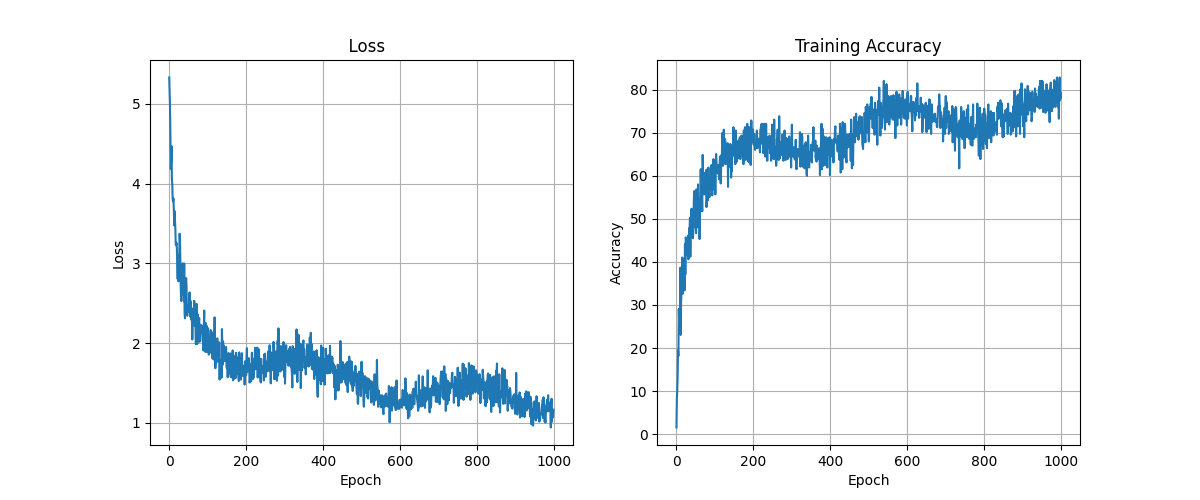
\includegraphics[width=1.0\linewidth]{images/loss_accuracy.png}
    \caption{Loss and Accuracy plot for SimClr}
    \label{fig:loss_accuracy}
\end{figure}

\subsection{Relax}
Our SimCLR trained model is used as a feature extractor for the RELAX\cite{wickstrom2023relax} model. Masks are generated for the input image and simlarity is found between the masked image and the original image. Importance and uncertainty are calculated for each pixel in the image using simlarity scores.

Figure \ref{fig:result1}, \ref{fig:result2}, and \ref{fig:result3} show the RELAX explanation and uncertainty on CIFAR-10 dataset. In the figure \ref{fig:result2}, model is able to give importance to the aeroplane in the image and uncertainty is high in the background. In the figure \ref{fig:result3}, model is able to give importance to the bird in the image and uncertainty is high in the background. This shows that RELAX model is able to give importance to the object in the image and uncertainty in the background. 
\begin{figure}[h]
    \centering
    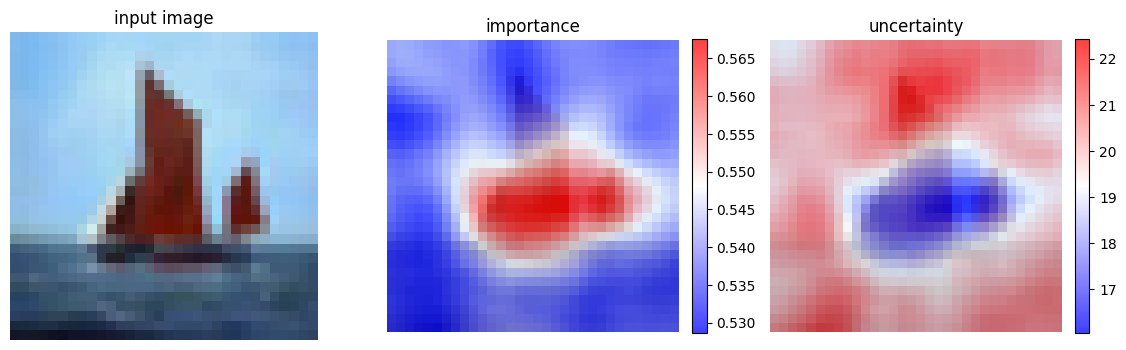
\includegraphics[width=1.0\linewidth]{images/Result1.png}
    \caption{RELAX explanation and uncertanity on CIFAR-10 dataset}
    \label{fig:result1}
\end{figure}
\begin{figure}[h]
    \centering
    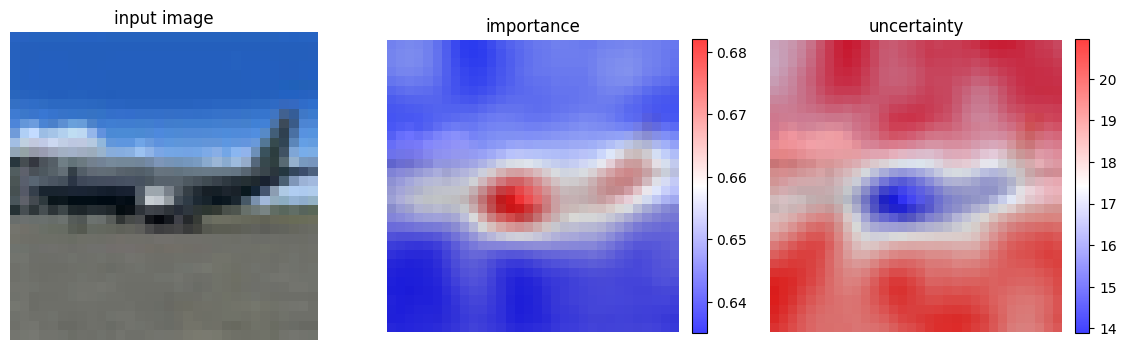
\includegraphics[width=1.0\linewidth]{images/Result2.png}
    \caption{RELAX explanation and uncertanity on CIFAR-10 dataset}
    \label{fig:result2}
\end{figure}
\begin{figure}[h]
    \centering
    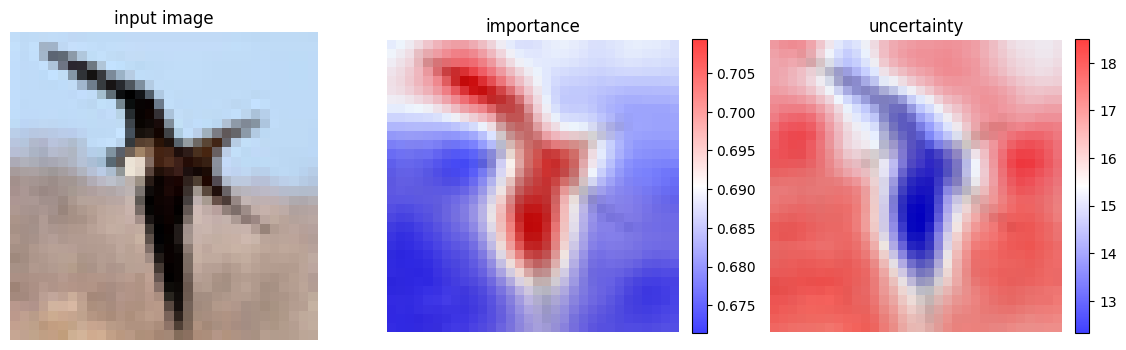
\includegraphics[width=1.0\linewidth]{images/Result3.png}
    \caption{RELAX explanation and uncertanity on CIFAR-10 dataset}
    \label{fig:result3}
\end{figure}
